\chapter{Infraestructura Software} 

Una vez presentados los objetivos que tenemos marcados hay que echar una mirada a las tecnologías software que tenemos disponibles para utilizarlas como base y pilares del proyecto. La más importante y sobre la que está centrado el proyecto es WebRTC. Luego utilizaremos, como apoyo para cubrir las partes que WebRTC no llega, ICEJS junto con la infraestructura que tiene ya desarrollada JdeRobot.


\section{WebRTC}

Web Real-Time Communication (WebRTC) es un proyecto opensource y gratuito que nos permite tener en el navegador tecnología en tiempo real ('Real-Time Communication' ó RTC), sin plugins, a través de una simple API de JavaScript. Facilita las llamadas de voz, videollamadas, chat y compartimiento de archivos y datos. WebRTC es una tecnología Peer-to-Peer, por lo que nos permite desarrollar estas aplicaciones para que funcionen directamente desde un navegador a otro \textbf{sin pasar por servidor intermedio.} \\

En todo el documento nos referimos a una llamada WebRTC entre dos navegadores, lo cual es su principal propósito, pero también esta diseñado para que pueda ser integrado con otros sistemas de comunicación como voz sobre IP (VOIP), clientes SIP, e incluso sobre la red telefónica pública conmutada (PSTN).\\

Enviar audio y/o vídeo con calidad, e intercambiar cualquier tipo de datos requiere de muchas funcionalidades complejas en el navegador. Para no preocuparnos de estas dificultades la API de WebRTC nos proporciona todo el set completo de funciones para manejar y crear nuestras aplicaciones, como el control y administración de la conexión, codificación/decodificación del audio/vídeo, negociación entre navegadores, control de la conexión, firewall y NAT traversal.\\

Con unas docenas de lineas de JavaScript podemos tener una videconferencia Peer-2-Peer con intercambio de archivos o datos en tiempo real. Ese es el potencial que WebRTC tiene. Pero aún así hay una serie de escollos como señalización, descubrimiento de peers, negociación de la conexión o seguridad que debemos controlar para conseguir una llamada exitosa.\\

Que WebRTC no necesita un servidor no es del todo cierto, ya que sí que necesita de lo que llamamos Servidor de Señalización. Este es el encargado de establecer el primer contacto entre ellos, facilitando el intercambio de paquetes de la negociación WebRTC.\\

WebRTC está compuesto de 3 API's:

\begin{itemize}
\item getUserMedia: adquisición del streaming de audio y video.
\item RTCPeerConnection: comunicación de audio y video.
\item RTCDataChannel: comunicación de cualquier otro tipo de datos.
\end{itemize}

A continuación vamos a desgranar y explicar como funciona el intercambio de paquetes de señalización así como cada una de las API's que componen WebRTC.\\

\begin{center}
\fbox{\begin{varwidth}{\dimexpr\textwidth-2\fboxsep-2\fboxrule\relax}
\textbf{\underline{\emph{Nota:}}} En este momento WebRTC es accesible para todos los usuarios a través de navegadores como Chrome o Firefox. Sin embargo, WebRTC está aún en construcción, tanto la forma de implementar las API's que tiene cada navegador como la propia norma, con sus protocolos de funcionamiento. Como resultado tenemos que todo lo que exponga sobre estas API's puede cambiar en el futuro.
\end{varwidth}}
\end{center}


\subsection{Señalización} 
\label{subsec:senalizacion}

Señalización es el proceso de intercambio de datos y metadatos necesarios para coordinar una llamada entre navegadores con WebRTC. Para realizar esta labor WebRTC necesita de la ayuda de un servidor externo ya que la norma deja el campo de la señalización a la capa de la aplicación.\\

Entre las labores de la señalización se encuentran la detección de los peers, el intercambio de paquetes de control de la sesión como los \textit{ICE candidates} y los \textit{SDP (Session Description Protocol)}, las prestaciones que puede darnos cada peer así como cualquier otro dato o paquete necesario para realizar este 'apretón de manos' inicial.\\

WebRTC no especifica que tipo de servidor hemos de usar para estas funciones. Esto es debido a que diferentes aplicaciones pueden preferir diferentes servidores básicos o personalizados según sus necesidades. La única restricción es el uso de la arquitectura JSEP, la cuál especifica cómo debe ser la secuencia de señalización para tener una llamada exitosa.

\subsubsection{Arquitectura \textit{JSEP (JavaScript Session Establishment Protocol)}}

El servidor debe usar la arquitectura JSEP. Esta arquitectura elimina al navegador de casi todo el flujo de señalización, el cual se maneja desde JavaScript haciendo uso de dos interfaces: transfiriendo los SDP local/remoto e interactuando con la maquina de estados ICE. Esta arquitectura nos evita, entre otras cosas, que el navegador tenga que guardar estados de sesión, de tal manera que se pueden guardar en el servidor y evitar problemas si la página se recarga, por ejemplo. \\

Como ya hemos comentado, JSEP no establece un modelo particular de señalización más allá de usar uno capaz de realizar el intercambio de los SDP y ICE según la norma RFC3264 de oferta/respuesta, de tal manera que ambas partes de la llamada sepan como actuar en cada momento. JSEP nos da los mecanismos necesarios para crear estas ofertas, así como aplicarlas a las sesión.\\

El orden en que se llaman a estas mecanismos o funciones de la API es importante, por lo que la aplicación deberá saber el orden en el que tiene que llamar a cada una, convertir las ofertas en mensajes que entienda el protocolo de señalización elegido y hacer la conversión inversa con los mensajes que se reciben para obtener ofertas que entiendan as API's.\\

El manejo de las \textit{session descriptions} es simple y sencillo. Siempre que el intercambio de una oferta/respuesta es necesario, el peer que establece la llamada ó \textit{caller} crea la oferta llamando a la función \emph{createOffer()} de la API. Esta oferta puede ser modificada por la aplicación si así fuese necesario y se establece como configuración local en ese peer con \emph{setLocalDescription()} y se envía al peer remoto a través del servidor de señalización utilizado. Al recibir esta oferta el peer \textit{called} lo utiliza como configuración del otro peer con \emph{setRemoteDescription()} y utiliza \emph{createAnswer()} para crear una respuesta apropiada, la cual establece como configuración local (\emph{setLocalDescription()}) y envía la respuesta de vuelta a través del servidor de señalización. El caller al recibir la respuesta llama también a \emph{setRemoteDescription()}, y de esta manera ambos lados tienen la información del media propia y la del peer remoto.\\


\subsubsection{Descriptores de Sesión y Máquina de Estados}

Para establecer un intercambio de media, el \textit{user agent} del navegador necesita parámetros específicos para indicar al peer remoto qué es lo que va a transmitir, de la misma manera que necesita saber el media que va a recibir para saber como decodificarlo y manejarlo. Estos datos se determinan en la descripción de sesión (SDP), los cuales se intercambian en ofertas/respuestas usando las API's JSEP como ya hemos visto anteriormente.\\

Si el SDP pertenece a la parte local o remota tiene su importancia. Una vez realizado el intercambio, cada parte mirará la lista de codecs soportados por él mismo y por la otra parte, y el cruce de los resultados determinará que codecs debe enviar y cuál espera recibir. Como podemos intuir, los parámetros exactos de la transmisión solo se pueden saber una vez la oferta y la respuesta han sido intercambiados. Sin embargo, hay ocasiones en las que el caller o el que hace la oferta puede recibir media después de enviar esta pero antes de recibir la respuesta de la otra parte. Para procesar este media de manera adecuada, el manejador de caller debe conoce los detalles de la oferta antes de que la respuesta llegue.\\

Por lo tanto, para manejar los session description de manera correcta, los user agent necesitan:

\begin{itemize}
\item Conocer si el session description pertenece a la parte local o remota.
\item Conocer si el session description es una oferta o una respuesta.
\item Permitir a la oferta ser especificada independientemente de la respuesta.
\end{itemize}

Para satisfacer estas premisas JSEP aborda esto añadiendo los métodos setLocalDescription() y setRemoteDescription() y teniendo un campo en los session description indicando el tipo de sesión que se suministra.\\

JSEP también permite el uso de respuestas provisionales. Estas respuestas permiten al peer remoto o called comunicar e informar de los parámetros iniciales de la sesión al caller, de tal manera que la sesión puede comenzar mientras se espera una respuesta final posteriormente. Este concepto es importante en el modelo oferta/respuesta, ya que al recibir una de estas respuestas el caller puede liberar y usar más recursos como extra \textit{ICE candidates, TURN candidates} o vídeo decodecs. Estas respuestas provisionales no provocan ningún tipo de des-asignación o problema, por lo que pueden ser recibidas a lo largo de la llamada para estabilizar o mejorar la misma según varíen las condiciones del ancho de banda de uno de los peers, por ejemplo.\\


DIAGRAMAS CON LA MAQUINA DE ESTADOS (pagina rtcweb-wg.github.io)
LISTA DE CODECS PERMITIDOS



http://www.html5rocks.com/en/tutorials/webrtc/infrastructure/
https://www.webrtc-experiment.com/docs/WebRTC-Signaling-Concepts.html

\subsubsection{Formato de los Descriptores de Sesión}

En la especificación WebRTC, los descriptores de sesión o session descriptions están formados por mensajes \textit{SDP (Session Description Protocol)}. Este formato no es el más óptimo para manipular con JavaScript, pero es el más popular y aceptado en el campo de las comunicaciones audiovisuales en tiempo real. Este formato es el que usa JSEP para formar e intercambiar los descriptores de sesión.\\

Para facilitar el procesado en JavaScript y una futura flexibilidad, los SDP nos los genera la API como un objeto o \textit{blob}. Si en un futuro WebRTC soporta algún formato nuevo para los descriptores de sesión, estos serán fácilmente añadidos y habilitados para poder usarlos en nuestras aplicación en vez de SDP.\\

La forma que tiene un paquete SDP es la siguiente:

\begin{lstlisting}[caption=Ejemplo paquete SDP]
v=0
o=- 7729291447651054566 1 IN IP4 0.0.0.0
s=-
t=0 0
a=group:BUNDLE a1 d1
a=ice-options:trickle
m=audio 9 UDP/TLS/RTP/SAVPF 96 0 8 97 98
c=IN IP4 0.0.0.0
a=rtcp:9 IN IP4 0.0.0.0
a=mid:a1
a=msid:QI39StLS8W7ZbQl1sJsWUXkr3Zf12fJUvzQ1
       QI39StLS8W7ZbQl1sJsWUXkr3Zf12fJUvzQ1a0
a=sendrecv
a=rtpmap:96 opus/48000/2
a=rtpmap:0 PCMU/8000
a=rtpmap:8 PCMA/8000
a=rtpmap:97 telephone-event/8000
a=rtpmap:98 telephone-event/48000
a=maxptime:120
a=ice-ufrag:7sFvz2gdLkEwjZEr
a=ice-pwd:dOTZKZNVlO9RSGsEGM63JXT2
a=fingerprint:sha-256 6B:8B:F0:65:5F:78:E2:51:3B:AC:6F:F3:3F:46:1B:35
                     :DC:B8:5F:64:1A:24:C2:43:F0:A1:58:D0:A1:2C:19:08
a=setup:active
a=rtcp-mux
a=rtcp-rsize
a=extmap:1 urn:ietf:params:rtp-hdrext:ssrc-audio-level
a=extmap:2 urn:ietf:params:rtp-hdrext:sdes:mid
a=ssrc:4429951804 cname:Q/NWs1ao1HmN4Xa5

m=application 9 UDP/DTLS/SCTP webrtc-datachannel
c=IN IP4 0.0.0.0
a=mid:d1
a=fmtp:webrtc-datachannel max-message-size=65536
a=sctp-port 5000
a=fingerprint:sha-256 6B:8B:F0:65:5F:78:E2:51:3B:AC:6F:F3:3F:46:1B:35
                     :DC:B8:5F:64:1A:24:C2:43:F0:A1:58:D0:A1:2C:19:08
a=setup:active
\end{lstlisting}


\subsubsection{Interactive Connectivity Establishment (ICE)}

Al igual que los peer tienen que intercambiar información sobre el media, también necesitan hacerlo sobre la información de \textit{network} para que los peer sean visibles entre ellos y puedan alcanzarse. ICE es una técnica usada en aplicaciones de voz, vídeo, peer-2-peer, entre otros que nos permite solucionar problemas de alcance de red entre dos ordenadores. Estos problemas son debidos a que los ordenadores suelen estar dentro de una red privada y/o firewall. Esta técnica nos permite descubrir suficiente información sobre la topología de los otros peer para encontrar una o varias rutas potenciales entre ellos.\\

Esta información ha de obtenerse de manera local en cada peer con el \textit{ICE Agent} asociado a cada objeto RTCPeerConnection. El ICE Agent es responsable de: 

\begin{itemize}
\item Reunir tuplas candidatas de IP + Puerto.
\item Realizar pruebas de conectividad entre los peers.
\item Enviar \textit{keepalives}.
\end{itemize}

Una vez se ha finalizado y configurado el proceso de session description, el ICE Agent local comienza automáticamente el proceso de descubrir todos los posibles candidatos en el peer local. Cada candidato posible se le llama \textit{ICE Candidate}:

\begin{enumerate}
\item El ICE Agent pide al sistema operativo las direcciones IP locales.
\item Consulta a un servidor \emph{STUN (Session Traversal Utilities for NAT}) externo la tupla de dirección IP pública y puerto del peer.
\item Consulta a un servidor \emph{TURN (Traversal Using Relays around NAT)} como último recurso. 
\end{enumerate}

Como podemos ver, ICE necesita de servidores externos para obtener la tupla de dirección IP y puerto públicos necesarios para el otro peer si esta fuera de la misma red local. STUN  es un protocolo estandarizado para descubrir direcciones IP publicas de equipos que están detrás de un NAT. TURN es un servidor para transmitir mensajes entre dos clientes. Este servidor solo se usará si falla la conexión Peer-2-Peer después de probar con las direcciones IP locales y las públicas obtenidas en el servidor STUN. No es obligatorio configurar estos servidores. Si la conexión entre los peer es en la misma red no necesitamos configurar servidores STUN/TURN ya que con las direcciones locales es suficiente.\\

DIAGRAMA DE ESTADOS DE ICE (PAGINA 132 (118) DEL LIBRO DE WEBRTC)

Como podemos ver en la figura, cada vez que el navegador recolecta un nuevo ICE Candidate, la función \textit{handleIceCandidate(}) se activa y es la encargada de enviar el candidato al peer remoto a través del servidor.\\
 
Cuando un ICE Candidate llega al peer remoto, se añade en RTCPeerConnection la información de sesión que ontiene ese paquete con \textit{setRemoteDescription()}, de tal manera que el ICE Agent puede empezar a hacer pruebas de conectividad para ver si puede alcanzar al otro peer.\\

Una vez los dos ICE Agent tienen una lista completa de los ICE Candidates de ambos peers, cada agente comprueba pareando ambas lista cuales funcionan. Para ello tienen una planificación de prioridades: primero direcciones IP locales, luego IP públicas y finalmente si ambas fallan servidor TURN. Cada comprobación es una peticion/respuesta STUN que el cliente realiza con un particular candidato enviando una petición STUN desde el candidato local al candidato remoto.\\

Si uno de los pares de candidatos funciona, entonces tenemos una ruta de conexión entre ambos peer. Si todos los candidatos fallan ambas conexiones RTCPeerConnection se marca como fallida o la conexión se hace a través de un servidor TURN.\\

Cuando una conexión se ha establecido correctamente cada ICE Agent continua haciendo peticiones STUN periódicas al otro peer, lo cual sirve también como \textit{keepalives}.\\

\begin{normalsize}
\noindent \textbf{ICE Candidate Trickling}\\
\end{normalsize}

Recopilar IP's locales es rápido, pero conseguir las IP's publicas con sus puertos a través de servidores STUN requiere de un intercambio de paquetes entre el peer y el servidor STUN y por consiguiente más tiempo.\\

ICE Candidate Tricking es una extensión del protocolo ICE por la cuál el caller puede incrementar el número de candidatos para el called después de la primera oferta. Este proceso permite al called comenzar a establecer las conexiones ICE por encima de la llamada inmediatamente, sin tener que esperar a que el caller recopile todos los posibles candidatos. Con esta técnica conseguimos un establecimiento del media más rápido.\\

Esta técnica es opcional aunque es la recomendada. Las aplicaciones que lo soportan pueden enviar directamente la oferta SDP inicial sin candidatos ICE inmediatamente, y enviar candidatos individuales cuando los vayan descubriendo; las aplicaciones que no lo soportan simplemente esperan la indicación de que el \textit{gathering} está completo, crean la oferta con todos los candidatos y enviarla.\\

\begin{enumerate}
\item Intercambio ofertas SDP sin ICE Candidates.
\item Cuando se descubre un candidato se envía directamente a través del servidor de señalización.
\item La comprobación de los ICE Candidates se realiza en el momento de recibir uno.
\end{enumerate}

\begin{normalsize}
\noindent \textbf{Formato de un ICE Candidate}\\
\end{normalsize}

\begin{lstlisting}[caption=Ejemplo paquete SDP]
candidate:1 1 UDP 1694498815 192.0.2.33 10000 typ host
\end{lstlisting}

\noindent \textbf{Fundación (1):} Identificador para cada candidato del mismo tipo, misma interfaz y servidor STUN.\\
\textbf{ID (1):} Identificador. 1 para RTP, 2 para RTCP.\\
\textbf{Protocolo (UDP):} Protocolo de transporte del candidato.\\
\textbf{Prioridad (1694498815): }Prioridad del componente dado.\\
\textbf{Dirección IP y puerto (192.0.2.33 10000): }Direccion IP y puerto del candidato.\\
\textbf{Tipo (typ):} Tipo del componente.\\
\textbf{Dirección relacionada (host):} Información opcional que contiene dirección IP y puerto privado.\\

\subsubsection{Negociación de Vídeo}

La negociación de vídeo es un proceso a través del que el cada peer puede indicar al otro que resoluciones y \textit{frames rate} de vídeo es capaz de recibir. Esto lo hace a través de un atributo \textit{'a=imageattr'} en el SDP. Cada peer puede tener limites como la capacidad de proceso que el decoder tiene, o simplemente restricciones de la aplicación.\\


\subsection{WebRTC API's}

\subsubsection{getUserMedia} 

getUserMedia es la API encargada de suministrarnos el streaming de audio y/o vídeo. Pide permiso al usuario para acceder y utilizar los dispositivos hardware como la cámara y el micrófono. Por el momento solo esta disponible para captar el hardware de audio y vídeo anteriormente mencionado, pero se pretende mejorar y ampliar la API para que en un futuro se pueda hacer streaming de casi cualquier fuente de datos, como un disco duro o sensores conectados al ordenador.\\

Para tener una rica videoconferencia no es suficiente con obtener los streaming en formato \textit{raw} de la cámara o el micrófono. Cada streaming debe ser procesado para aumentar la calidad, sincronizarlos y ajustar el \textit{bitrate} de salida según las fluctuaciones del ancho de banda y la latencia entre peers. A la hora de recibir el streaming nos encontramos en la misma situación pero a la inversa. WebRTC nos da unos motores de procesado de audio y vídeo (figura \ref{fig:audio-video_engines}) que hará todas estas cosas por nosotros.\\

\begin{figure}[htb]
\centering
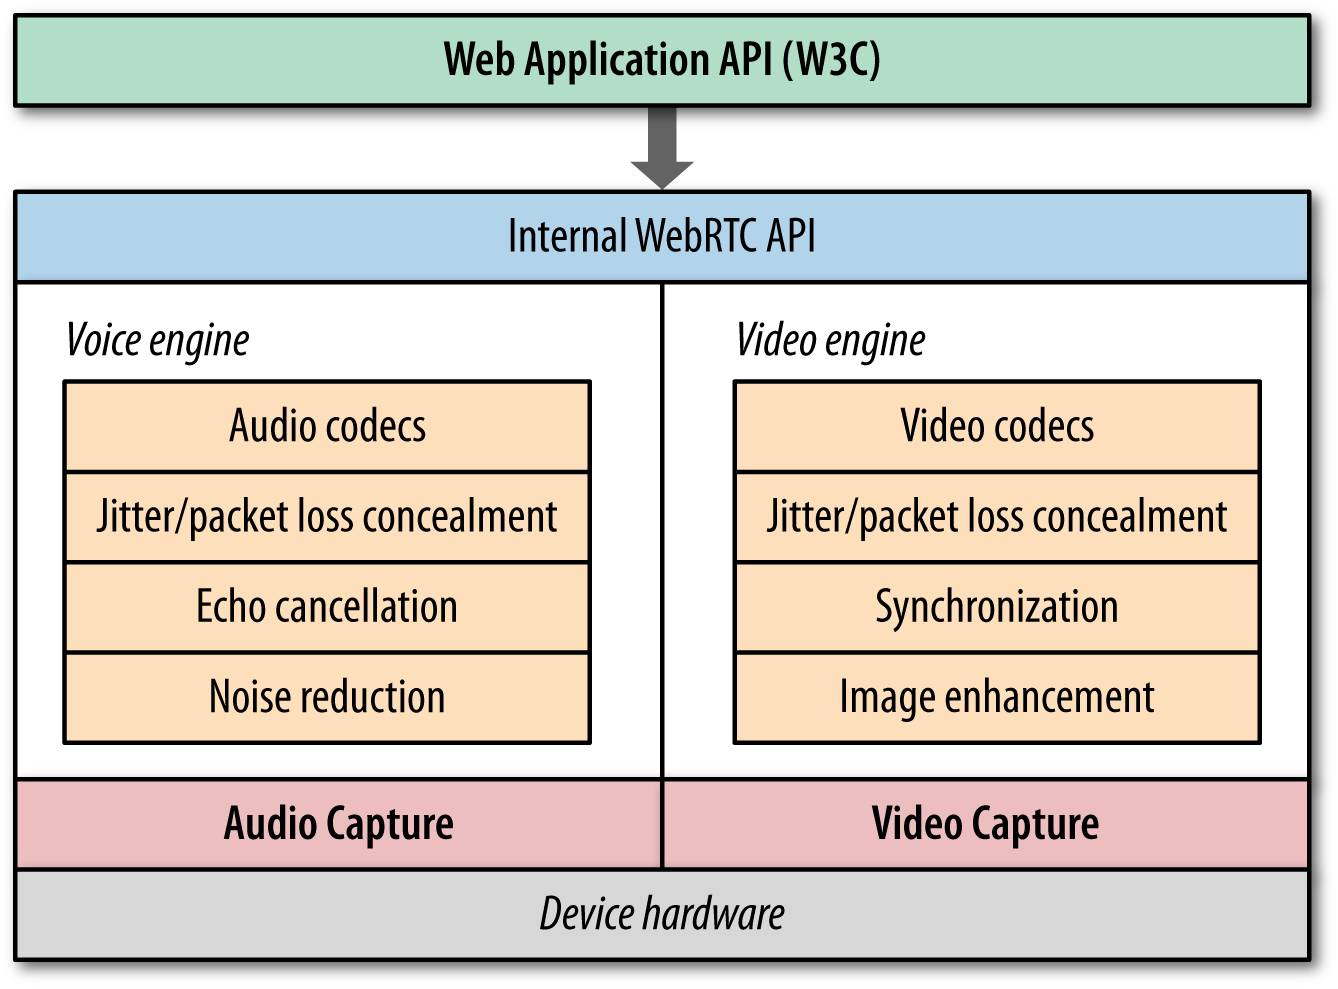
\includegraphics[width=0.9\textwidth]{audio-video_engines}
\caption{Motores de audio y video de WebRTC }
\label{fig:audio-video_engines}
\end{figure}

getUserMedia es la API que nos suministra las funciones y los motores necesarios para poder cumplir con las especificaciones anteriormente mencionadas, así como manipular o procesar los streaming obtenidos. El objeto \textit{MediaStream} (figura \ref{fig:mediaStream}) es la forma en la que nos suministra los streams esta API.\\

\begin{itemize}
\item El objeto MediaStream consiste en uno o varias pistas o \textit{tracks} (\textit{MediaStreamTrack}).
\item Las pistas que componen el MediaStream están sincronizadas una con la otra.
\item La salida del MediaStream puede ser enviada a uno o varios destinatarios, como fuente de vídeo local, un peer remoto o procesarlo con funcionalidades que nos proporciona, por ejemplo, HTML5.
\end{itemize}

\begin{figure}[htb]
\centering
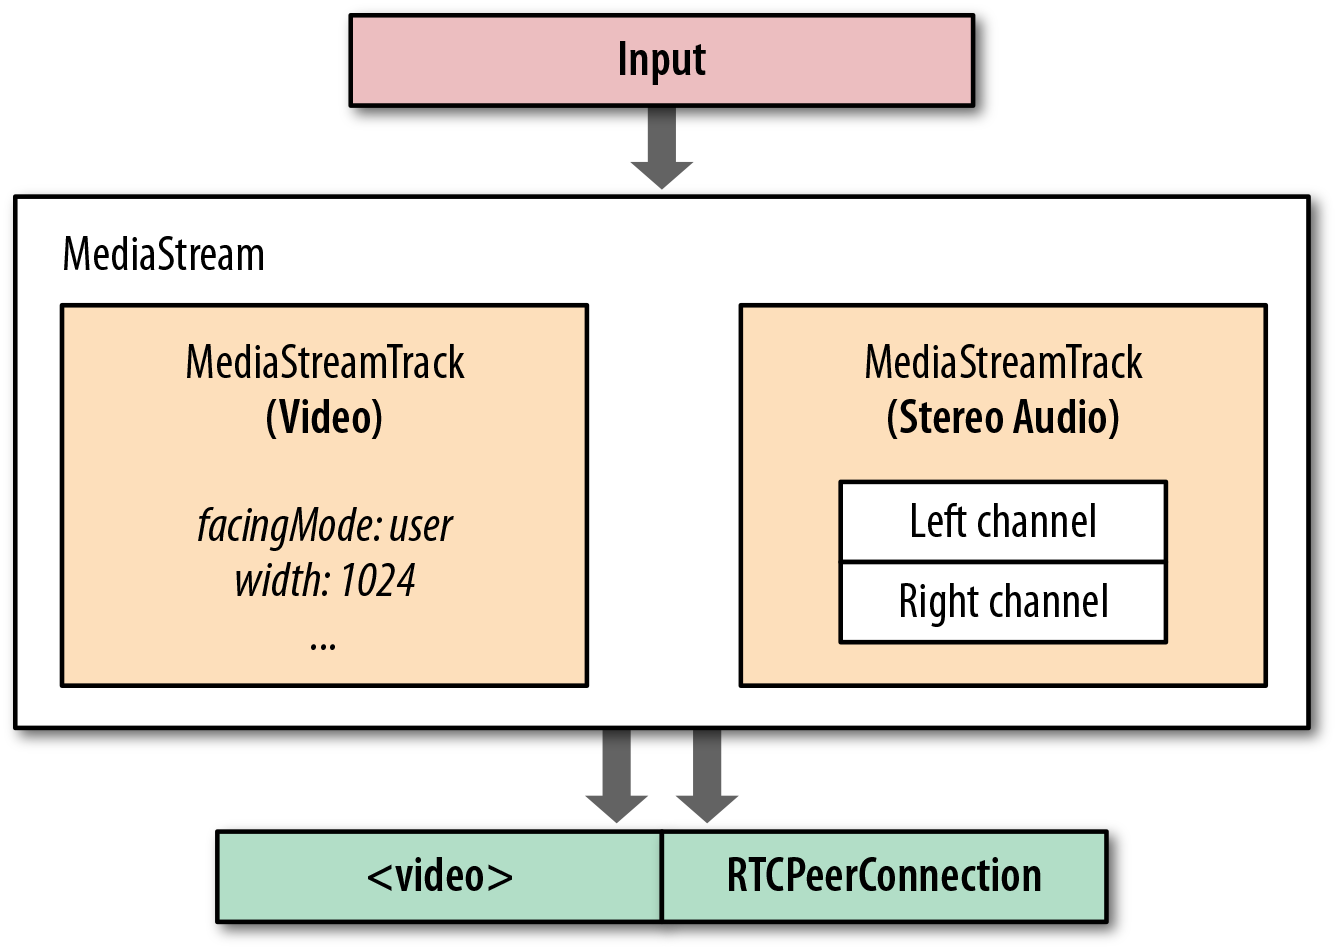
\includegraphics[width=0.9\textwidth]{mediaStream}
\caption{MediaStream}
\label{fig:mediaStream}
\end{figure}

Todo el procesado de audio y vídeo, como la cancelación de ruido, ecualización, mejora de la imagen y todas las demás son automáticamente manejadas por os motores de audio y vídeo.\\

Sin embargo, las características del media stream son restringidas por las capacidades de los dispositivos de entrada: audio mono o stereo, diferentes resoluciones de video según la cámara, etc. Cuando hacemos una petición de media al navegador, getUserMedia nos permite indicar una lista de restricciones obligadas y opcionales.\\

\begin{lstlisting}[caption=Llamada a función RTCPeerConnection]
var constraints = {
    audio: false,
    video: {
        width: { min: 1024, ideal: 1280, max: 1920 },
        height: { min: 576, ideal: 720, max: 1080 },
    }
};

navigator.getUserMedia(constraints, handleUserMedia, handleUserMediaError); 

function handleUserMedia(stream){
    var video = document.querySelector('video');
    video.src = window.URL.createObjectURL(stream);
}

function handleUserMediaError(error){
	console.log('getUserMedia error: ', error);
}

\end{lstlisting}

\subsubsection{RTCPeerConnection}

Esta API es la encargada de crear la conexión Peer-2-Peer entre el navegador local y el remoto. Trabaja de manera diferente si es el que hace la llamada (\textit{caller}) y el que la recibe (\textit{called}) debido a la señalización oferta/respuesta que ya hemos visto. Para ello hace uso de sus funciones para completar el proceso de señalización descrito anteriormente.\\

\noindent Es también la encargada de manejar la conexión una vez establecida. Entre las funciones automáticas que realiza se encuentran:\\

\begin{enumerate}
\item Ocultamiento de paquetes perdidos.
\item Cancelación de eco.
\item Adaptación del ancho de banda.
\item Buffer dinámico en función del jitter o delay.
\item Control automático de ganancia.
\item Reducción o eliminación de ruido.
\end{enumerate}

Es el desarrollador de la aplicación el encargado de llamar a las funciones que componen esta API en el orden, tiempo y forma correcta para cumplir con la arquitectura JSEP y conseguir un intercambio de descriptores de sesión y de ICE Candidates exitoso.\\

\noindent La función admite dos argumentos, los cuales son opcionales: 

\begin{lstlisting}[caption=Llamada a función RTCPeerConnection]
var PC = new RTCPeerConnection(ICEconfig, pcConstraints);
\end{lstlisting}

\textit{ICEConfig} es una variable la cuál contiene los datos necesarios para conectarse con el servidor STUN y TURN y poder hacer NAT Trasversal. \textit{pcConstraints} también es una variable a la que se le pueden añadir una serie de restricciones como \textit{RtpDataChannels}, la cuál estará obsoleta en futuras versiones y se dejará de usar. Esta variable está para futuras mejoras.\\

\begin{normalsize}
\noindent \textbf{Protocolos de transporte en tiempo real}\\
\end{normalsize}

El cerebro humano es muy bueno 'rellenando huecos' pero altamente sensible a los delays. Si perdemos unas muestras de audio o vídeo no nos afecta demasiado en la percepción de lo que estamos recibiendo, pero en cambio añade un delay al audio con respecto al vídeo y hará que ese material nos sea hasta molesto.\\

Por este motivo las aplicaciones de audio y vídeo en tiempo real están diseñadas para tolerar pérdidas intermitentes de paquetes perdidos. Los codecs pueden rellenar estos pequeños espacios que dejan los paquetes perdidos, muchas veces incluso con muy poco impacto con respecto a la imagen real. Una baja latencia y el \textit{'timeliness'} es mucho mas importante que la fiabilidad (reliability).\\

Este requerimiento de timeliness sobre la fiabilidad es la primera razón por la que el protocolo UDP es elegido para el envío de datos en tiempo real. TCP es fiable y tiene entrega ordenada de paquetes. Si uno de ellos se pierde, entonces TCP almacena los paquetes siguientes y para la retransmisión hasta que el paquete perdido es reenviado y recibido. En cambio UDP no garantiza la entrega de paquetes, el orden de entrega, ruta de los paquetes ni control de congestión de red.\\

WebRTC usa UDP como protocolo de transporte. Dadas las características de UDP, ¿podemos simplemente enviar cada paquete según llega y olvidarnos? no, ya que también necesitamos mecanismos para atravesar NAT's y firewalls, negociar los parámetros de cada stream, encriptar los datos de usuario, congestión de red... Para abastecer estas necesidades WebRTC tiene una lista de protocolos y servicios que trabajan por encima de UDP.\\

\begin{figure}[htb]
\centering
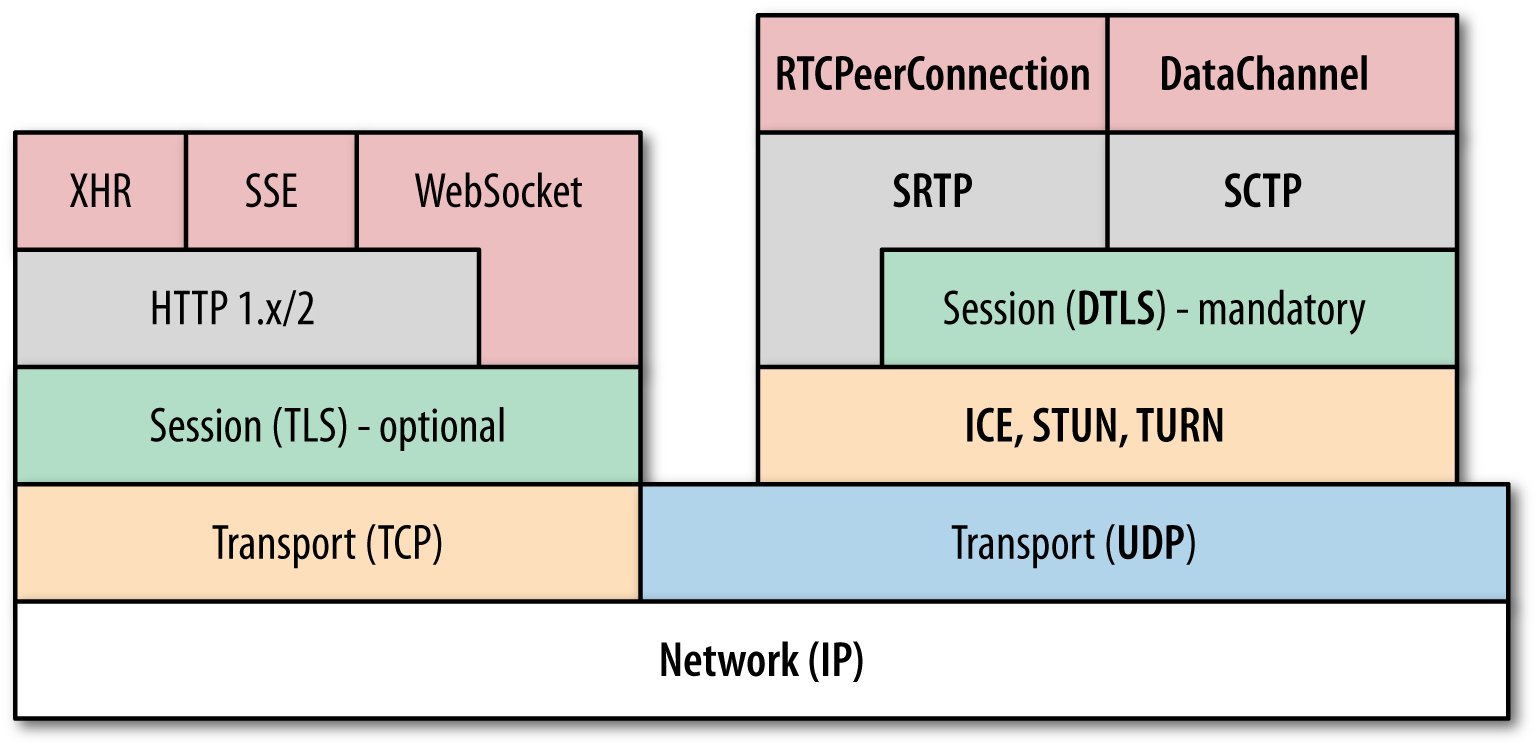
\includegraphics[width=0.9\textwidth]{pila_webrtc}
\caption{Pila de protocolos WebRTC}
\label{fig:pila_webrtc}
\end{figure}


ICE, STUN y TURN son necesarios para establecer y mantener la conexíon Peer-2-Peer sobre UDP, como ya hemos visto en el apartado de señalización.\\

\begin{normalsize}
\noindent \textbf{Entrega de vídeo con SRTP}\\
\end{normalsize}

WebRTC nos permite adquirir el video/audio y enviarlo para la visualización en el otro peer. También nos permite elegir las características con las que queremos adquirir ese video/audio, pero a partir de ahí es WebRTC y el motor de red el que se encarga del resto. Optimización en la codificacion, tratar con paquetes perdidos, jitter, etc, son algunas de las cosas con las que tiene que tratar WebRTC. Por este motivo WebRTC no garantiza la entrega en el otro peer del vídeo con a su máxima resolución.\\

El motor de red tiene su propio flujo de datos sin tener en cuenta desde el comienzo la capacidad de la red ni el bitrate del streaming. Primero empieza enviando el vídeo y el audio a un bitrate bajo (<500kbps) y luego comienza a ajustar la calidad del stream según la capacidad del ancho de banda. Según pueda variar el ancho de banda de la conexión de red así actúa el motor de red para ajustarlo.\\

SRTP define un formato de paquete estándar para enviar audio y vídeo a través de IP, pero por si mismo no proporciona ningún mecanismo o garantias de entrega en orden, fiabilidad en la entrega o corrección de errores. Simplemente encapsula el video y el audio con adicional metadata. Entre esta metadata cada paquete SRTP tiene un numero de secuencia incremental, una marca de tiempo y un identificador SSRC, lo que permite al peer que recibe el flujo detectar si los paquetes llegan desordenados, sincronizar los diferentes streams y asociar cada paquete al stream correspondiente.\\

SRTP usa un protocolo que lo complementa. Este es SRTCP, el cual es el protocolo que controla el numero de paquetes y bytes perdidos, ultimo numero de secuencia recibido, jitter de los paquetes SRTP recibidos y otras estadísticas. Periódicamente estas estadísticas se intercambian entre los peers y la usan para ajustar la tasa de envío, calidad de codificación y otros parámetros.\\

Ambos protocolos corren directamente sobre UDP y trabajan conjuntamente para adaptar y optimizar la conexión.\\


\subsubsection{RTCDataChannel}

Llegamos a la tercera y última pero no menos importante API de WebRTC. RTCDataChannel nos da la posibilidad de transferir todo tipo de datos u objetos a través de la conexión Peer-2-Peer establecida con RTCPeerConnection.\\

Esta conexión de datos es \textit{full duplex} y nos permite el intercambio de datos, intercambio de archivos, gaming, etc, todo ello con un delay mínimo y sabiendo de la salvaguarda de estos datos, ya que no pasan por ningún servidor intermedio sino que van de navegador a navegador. Las posibilidades son infinitas y se puede adaptar a cualquier necesidad que se tenga para nuestra aplicación.\\

\begin{normalsize}
\noindent \textbf{Capabilities}\\
\end{normalsize}

RTCDataChannel soporta un juego muy flexible de tipos de datos. Soporta \textit{strings}, binarios de JavaScript, \textit{Blobs}, \textit{ArrayBuffer} y \textit{ArrayBufferView}. Según nuestras necesidades nos puede resultar más útil un tipo de datos u otro.\\

Como protocolo de transporte soporta TCP, UDP y SCTP. Esto nos permite configurar la conexión de datos de manera \textit{reliable} o \textit{unreliable}. La primera de ellas nos garantiza la entrega de todos los mensajes que enviemos y que los mismos lleguen en el mismo orden que los hemos enviado. Esto provoca una sobrecarga que puede provocar un funcionamiento mas lento además de tener un mayor delay. La segunda de ellas no nos garantiza la entrega de todos los paquetes al otro peer, así como tampoco el orden en el que llegan. Esto reduce el \textit{overhead} permitiéndonos tener una conexión más rápida. SCTP es un protocolo de transporte similar a TCP y UDP que puede funcionar directamente en la cima del protocolo IP. Sin embargo, en WebRTC, SCTP es construido sobre un túnel DTLS, el cuál corre encima de UDP.

\begin{figure}[htb]
\centering
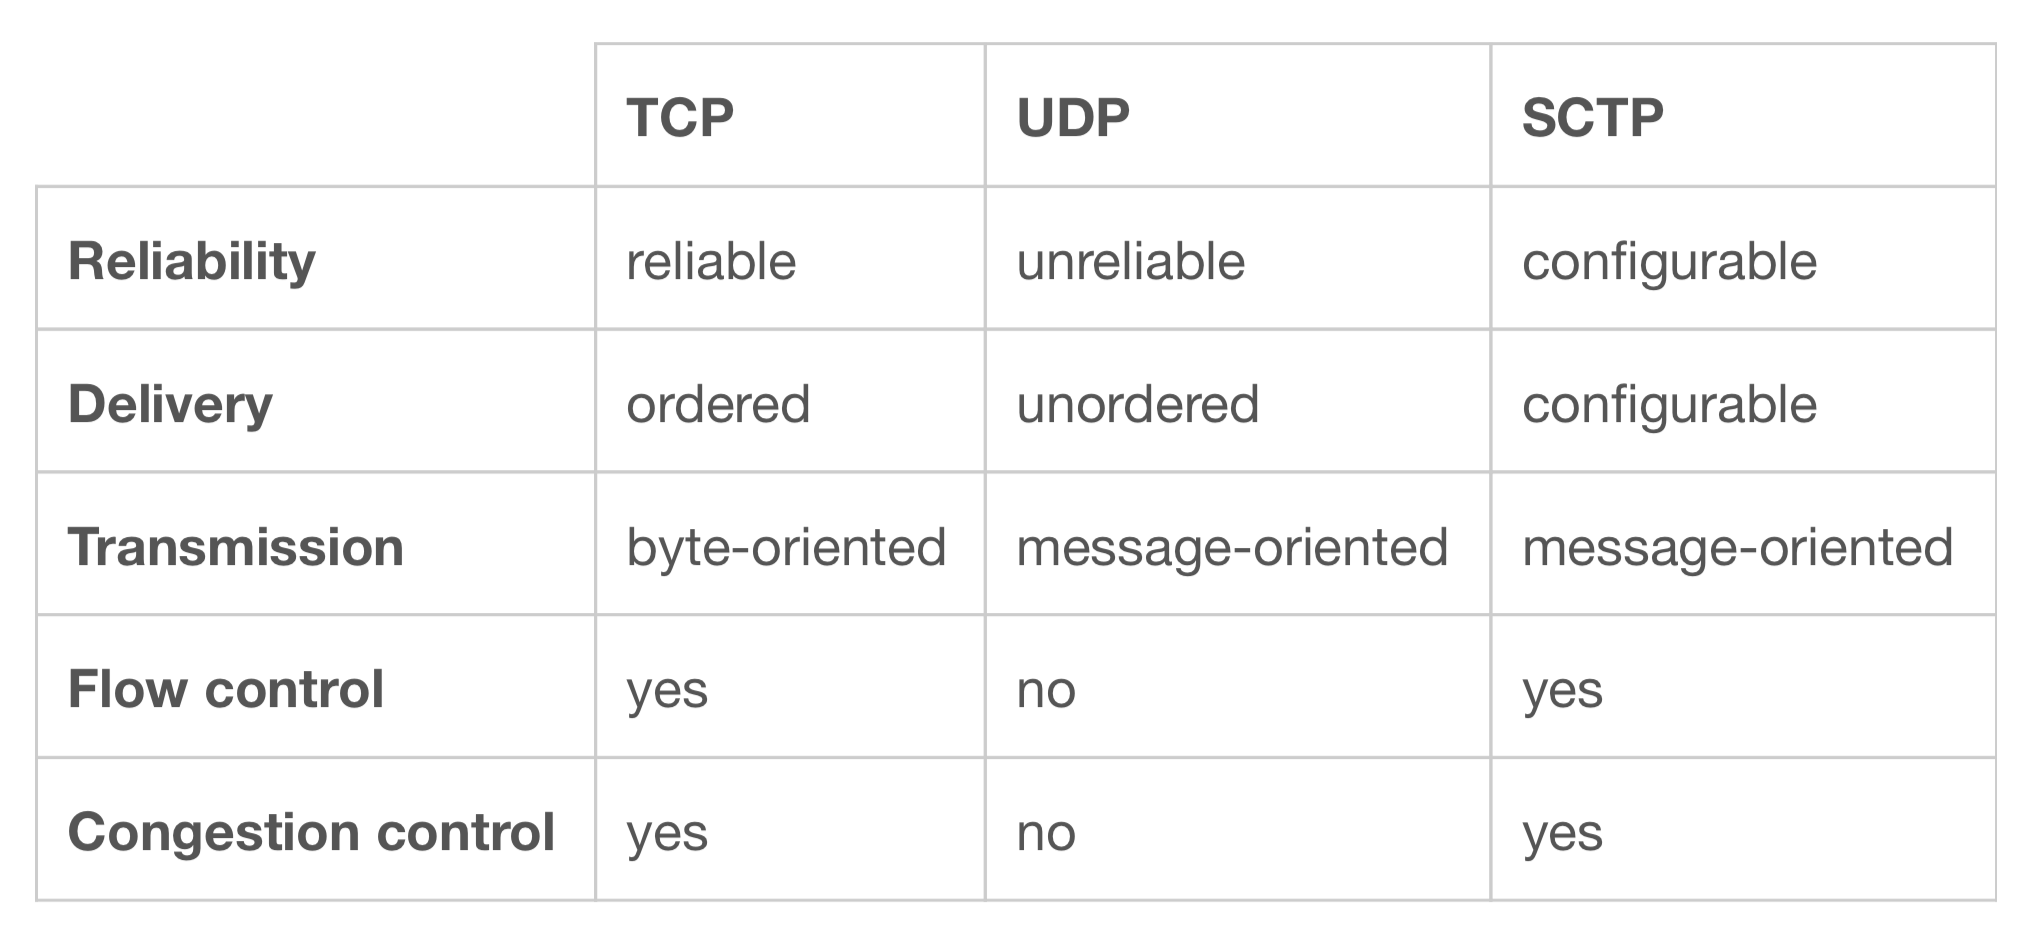
\includegraphics[width=0.9\textwidth]{RTCDataChannel_Capabilities}
\caption{RTCDataChannel Capabilities.}
\label{fig:datachannel_capabilities}
\end{figure}

\noindent Como las API's anteriores llamamos a RTCDataChannel con una variable con opciones de configuración:

\begin{itemize}
\item Ordered: Booleano para indicar si queremos que nos garantice la entrega ordenada de paquetes.
\item maxRetransmitTime: Tiempo máximo para intentar retransmitir cada paquete si la entrega falla. (Fuerza el modo \textit{unreliable}).
\item maxRetransmits: Número máximo de veces que queremos que reenvíe cada paquete si la entrega falla. No puede usarse junto con \textit{maxRetransmitTime}. (Fuerza el modo \textit{unreliable}).
\item Protocol: Permite el uso de un subprotocolo pero tiene que ser soportado por TCP/UDP.
\item Negociated: Si se configura en true, elimina la configuración automática del datachannel en el otro peer. Se da por echo que tienes previsto crear el canal de otra manera con el mismo ID.
\item Id: Permite dar tu propio ID al canal.
\end{itemize}

\begin{normalsize}
\noindent \textbf{Seguridad}\\
\end{normalsize}

La encriptación es un \textit{mandatory} (obligación) para todos los componentes WebRTC. Tanto audio, video, data e información de la aplicación debe estar encriptado cuando se transmite.. En RTCDatachannel todos los datos son codificados con \textit{Datagram Transport Layer Security (DTLS)}. DTLS es un derivado de SSL por lo que los datos que intercambies irán igual de seguro que si usásemos SSL. Es obligatorio, para que un navegador pueda usar WebRTC, que tenga implementado esta tecnología.\\


\begin{normalsize}
\noindent \textbf{Entrega de datos con SCTP}\\
\end{normalsize}

Como ya hemos visto en la imagen \ref{fig:pila_webrtc}, RTCDataChannel trabaja con un protocolo llamado \textit{Stream Control Transmission Protocol (SCTP)}, el cual corre sobre DTLS, y este a su vez corre sobre UDP. Recalco esto ya que a diferencia del audio y el vídeo, para enviar data de la aplicación si que necesitamos que lleguen todos los paquetes, por lo que si alguno se ha perdido hay que reenviarlo.\\

\noindent WebRTC requiere de 4 características que debe cumplir el protocolo:

\begin{enumerate}
\item El protocolo de transporte debe permitir tener varios canales independientes multiplexados.
\begin{enumerate}
\item Cada canal debe permitir entrega ordenada y desordenada.
\item Cada canal debe tener entrega fiable.
\item Cada canal debe tener niveles de prioridad definidos por la aplicación.
\end{enumerate}
\item El protocolo debe proveer 'orientado al mensaje', por lo que debe tener fragmentación y reagrupacion de los datos.
\item El protocolo debe tener mecanismos control del flujo y de la congestión.
\item El protocolo debe tener seguridad y confidencialidad en los datos que se envían.
\end{enumerate}

La última característica se cumple ya que SCTP corre sobre el túnel DTLS, por lo que los datos que enviemos van encriptados y seguros hasta nuestro destinatario. Por otro lado SCTP, como vemos en la tabla \ref{fig:datachannel_capabilities} permite configurar la fiabilidad y la entrega ordenada de paquetes. SCTP también trocea los datos que queremos enviar y los encapsula en paquetes SCTP de 224 bits.\\

Para el control de flujo y de congestión SCTP tiene un 'handshake' inicial similar al de TCP. Ambos usan la misma ventana inicial de congestión así como la misma lógica de crecimiento y decrecimiento para reducir la congestión una vez la comunicación está activa.\\


\section{ICE y ICEJS}

ICE o \textit{Internet Communication Engine} es un framework RPC orientado a objetos desarrollado por Zeroc con soporte para lenguajes como C++, C\#, Java, JavaScript, y Python entre otros, y SO's como Linux, Mac OS X y Windows, que nos permite crear conexiones e interacciones de red entre maquinas con servidores corriendo en diferentes lenguajes y/o SO's.\\

ICEJS, o ICE for JavaScript es un \textit{plugin} que se le puede añadir a ICE el cual añade la funcionalidad de \textit{websockets} lo que nos permite conectar navegadores a través de JavaScript a los protocolos comunes de ICE. \\

En versiones más actuales ICEJS viene incorporado en la suite principal de ICE, pero nosotros usaremos la versión 3.5 que es la que soporta la suite de JdeRobot, por lo que debemos instarlo una vez instalado ICE.\\

\section{JdeRobot}

JdeRobot es un proyecto de la Universidad Rey Juan Carlos. Es un framework para el desarrollo de aplicaciones relacionadas con la rebotica, la visión artificial, automatización del hogar y escenarios con sensores y actuadores, y software inteligente.\\

Esta suite tiene muchos complementos y componentes desarrollados, pero para este proyecto solo haremos uso de unos pocos:



\section{ArDrone de Parrot}

